\begin{frame}
\begin{itemize}
  \item $d-A^0$ a diagonal generic meromorphic connection
    \begin{itemize}
      \item abelian case is $n=1$
    \end{itemize}
  \item $A^0=dQ+\Lambda^0\frac{dz}{z}$ where
    \begin{itemize}
      \item $\Lambda^0$ is constant diagonal
      \item $Q=diag(q_1,\dots,q_n)$ diagonal matrix of meromorphic functions
    \end{itemize}
  \item $q_{ij}(z)=\text{leading Term of }q_i-q_j = \frac{a}{z^{k-1}}$ where
    \begin{itemize}
      \item $q_i-q_j = \frac{a}{z^{k-1}} + \frac{b}{z^{k-2}}+\dots$
      \item $\#\{q_{ij}\mid i \neq j\}=n^2-n$
      \item simple pole case is $k=1$
    \end{itemize}
  \end{itemize}
\end{frame}

\begin{frame}{Anti-Stokes directions}
Definition 3.2. The \emph{anti-Stokes} directions $\A\subset S^1$ are the
directions $d\in S^1$ such that for some $i \neq j$: $q_{ij}(z)\in\R_{<0}$ for
$z$ on the ray specified by $d$.
  \begin{center}
    \begin{tikzpicture}[scale=2]
      \node[label=below left:$0$] (zero) at (0,0) {};
      \fill (zero) circle (1pt);
      \draw[blue] (zero) circle (1cm);
      \draw[thick] (0,0) -- +({cos( 33 )},{sin( 33 )}) node[right] {d};
      \draw[thick] ({cos( 33 )},{sin( 33 )}) -- +({cos( 33 )},{sin( 33 )});
      \fill[blue!20!white] ({cos( 33 )},{sin( 33 )}) circle (1pt);

      \node[blue] at (-0.9,0.6) {$S^1$};
      \node at (-1.3,-0.7) {$\C$};
      \node at (2.2,.9) {ray specified by $d$};
    \end{tikzpicture}
  \end{center}
  \begin{itemize}
    \item We have $\frac{\pi}{k-1}$ rotational symmetry
      \begin{itemize}
        \item if $q_{ij}(z)\in\R_{<0}$ then
          $q_{ij}(z\exp(\frac{\pi\sqrt{-1}}{k-1}))\in\R_{<0}$
      \end{itemize}
    \item If $q_{ij}(z)\in\R_{<0}$ then $q_{ji}(z)\in\R_{>0}$
      \begin{itemize}
        \item in any arc $U \subset S^1$ subtending angle $\frac{\pi}{k − 1}$
          there are at most $\frac{n(n − 1)}{2}$ anti-Stokes directions.
      \end{itemize}
  \end{itemize}
\end{frame}

\begin{frame}{Anti-Stokes directions}
  \begin{center}
    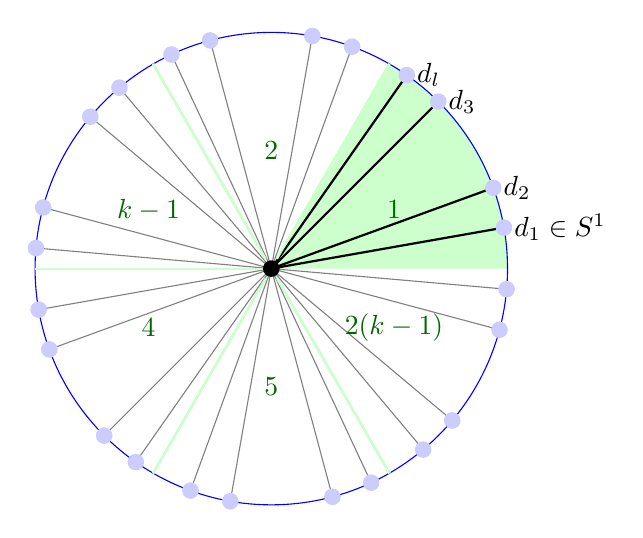
\begin{tikzpicture}[scale=3]
      \node[] (zero) at (0,0) {};
      \fill[fill=green!20!white] (0,0) -- (1,0) arc (0:60:1.0cm) -- cycle;
      \draw[blue] (zero) circle (1cm);

      \foreach \w/\str in {10/$d_1\in S^1$,
                           20/$d_2$,
                           45/$d_3$,
                           55/$d_l$}
      {\draw[thick] (0,0) -- +({cos( \w )},{sin( \w )}) node[right] {\str};
       \fill[blue!20!white] ({cos( \w )},{sin( \w )}) circle (1pt);
       \foreach \sep in {60,120,180,240,300}
       {\draw[green!20!white,thick] (zero) -- +({cos( \sep )},{sin( \sep )});
        \draw[gray] (0,0) -- +({cos( \w + \sep )},{sin( \w + \sep )});
        \fill[blue!20!white] ({cos( \w + \sep )},{sin( \w + \sep )}) circle (1pt);
       }
      };

      \foreach \sep/\str in {0/$1$
                            ,60/$2$
                            ,120/$k-1$
                            ,180/$4$
                            ,240/$5$
                            ,300/$2(k-1)$}
      {\node[green!40!black]
        at ({.6 * cos( \sep + 30 )},{.5 * sin( \sep + 30)}) {\str};
      };

      \fill (zero) circle (1pt);
    \end{tikzpicture}
  \end{center}

  \begin{itemize}
    \item
      
\begin{tikzpicture}[scale=3]
        \fill[blue!20!white] (0,0) circle (1pt);
      \end{tikzpicture}
      $\in\A\subset S^1$ and $\#\A=:r$
      \begin{itemize}
        \item is divisible by $2(k-1)$ \Rightarrow $l:=\frac{r}{2k-2}$
      \end{itemize}
    \item $\textbf{d}=(d_1,d_2,d_3,d_l)\subset\A$ is a half-period
  \end{itemize}
\end{frame}

\begin{frame}{Defns}
  \begin{itemize}
    \item $\Roots(d)=\{(ij)\mid g_{ij}(z)\in \R_{<0} \text{ along } d \}$
    \item The \emph{multiplicity} $\Mult(d)$ of $d$ is the number of roots
      supporting $d$.
    \item The group of \emph{Stokes factors} associated to $d$ is the group
    \[
      \mathbb{S}to_d(A^0) := \{K \in G \mid (K)_{ij}
        =\delta_{ij} \text{ unless } (ij) \text{ is a root of } $d$\}.
    \]
    \begin{itemize}
      \item $i=j$ \Rightarrow $(ij)$ is not a root of $d$. There are $1$nes on
        the diagonal.
      \item is a unipotent subgroup of $G=GL_n(\C)$ of dimension equal to the
        multiplicity of $d$
    \end{itemize}
    \item $n(n-1)/2=\Mult(d_1)+\dots+\Mult(d_l)$
  \end{itemize}
\end{frame}

\begin{frame}{Sectors}
  \begin{center}
    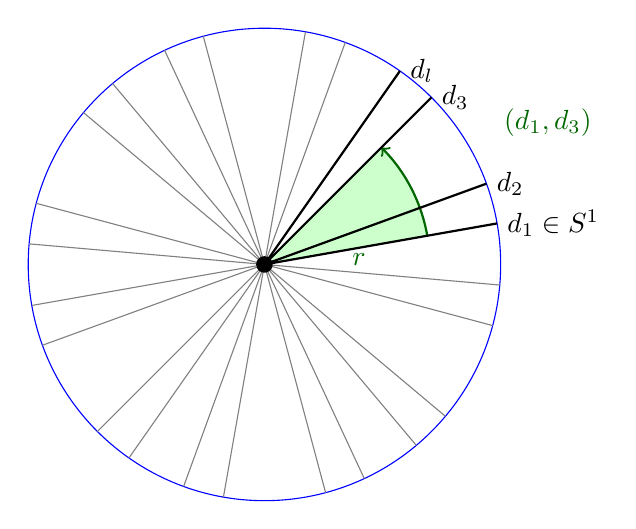
\begin{tikzpicture}[scale=3]
      \node[] (zero) at (0,0) {};
      \draw[blue] (zero) circle (1cm);
      \fill[fill=green!20!white]
        (0,0) -- +({cos(10) * 0.7},{sin(10) * 0.7}) arc (10:45:0.7cm) -- cycle;
      \draw[->,thick,green!40!black] ({cos(10) * 0.7},{sin(10) * 0.7}) arc (10:45:0.7cm);

      \foreach \w/\str in {10/$d_1\in S^1$,
                           20/$d_2$,
                           45/$d_3$,
                           55/$d_l$}
      {\draw[thick] (0,0) -- +({cos( \w )},{sin( \w )}) node[right] {\str};
       \foreach \sep in {60,120,180,240,300}
       {\draw[gray] (0,0) -- +({cos( \w + \sep )},{sin( \w + \sep )});}
      };

      \fill (zero) circle (1pt);

      \node[green!40!black] at (1.2,0.6) {$\Sect(d_1,d_3)$};
      \node[green!40!black] at (0.4,0.02) {$r$};

    \end{tikzpicture}
  \end{center}
  \begin{itemize}
    \item open
    \item The radius \textcolor{green!40!black}{$r$} will be taken sufficiently
    small when required later.
  \end{itemize}
\end{frame}

\begin{frame}
  $(ij)$ is a root of some $d\in\textbf{d}$ \Leftrightarrow
  $\frac{e^{q_i}}{e^{q_j}}\overset{z\to0}{\longrightarrow}0$ as along the ray
  $\textcolor{yellow!60!black}{\theta(\textbf{d})}\in S^1$ bisecting
  $\Sect(d_1,d_l)$
  \begin{center}
    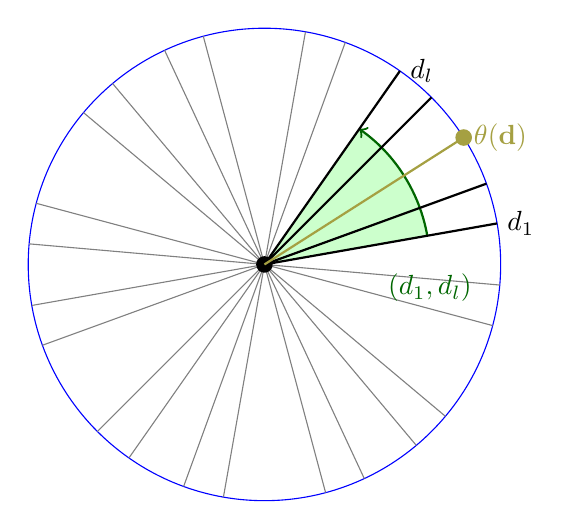
\begin{tikzpicture}[scale=3]
      \node[] (zero) at (0,0) {};
      \draw[blue] (zero) circle (1cm);
      \fill[fill=green!20!white]
        (0,0) -- +({cos(10) * 0.7},{sin(10) * 0.7}) arc (10:55:0.7cm) -- cycle;
      \draw[->,thick,green!40!black] ({cos(10) * 0.7},{sin(10) * 0.7}) arc (10:55:0.7cm);

      \foreach \w/\str in {10/$d_1$,
                           20/,
                           45/,
                           55/$d_l$}
      {\draw[thick] (0,0) -- +({cos( \w )},{sin( \w )}) node[right] {\str};
       \foreach \sep in {60,120,180,240,300}
       {\draw[gray] (0,0) -- +({cos( \w + \sep )},{sin( \w + \sep )});}
      };

      \fill (zero) circle (1pt);

      \node[green!40!black] at (0.7,-.1) {$\Sect(d_1,d_l)$};

      \draw[thick,yellow!60!black] (0,0) -- +({cos( 32.5 )},{sin( 32.5 )})
        node[right] {$\theta(\textbf{d})$};
      \fill[yellow!60!black] ({cos( 32.5 )},{sin( 32.5 )}) circle (1pt);

    \end{tikzpicture}
  \end{center}
  \textcolor{red}{Should that be $\Sect(d_i,d_j)$?}
\end{frame}

\begin{frame}{Ordering on a half-period}
  \[
    q_i\underset{\textbf{d}}{<}q_j \qquad :\Leftrightarrow
      \qquad (ij) \text{ is a root of some } d\in\textbf{d}
  \]
  Define permutation Matrix $P\in G$ associated do $\textbf{d}$ given by
  $(P)_{ij}=\delta_{\pi(i)j}$ where
  \begin{itemize}
    \item $\pi$ is the permutation of $\{1,\dots,n\}$ corresponding to
    \[
      q_i\underset{\textbf{d}}{<}q_j \qquad \Leftrightarrow \qquad \pi(i)<\pi(j)
    \]
  \end{itemize}
\end{frame}

\begin{frame}{Lemma 3.2}
  \begin{enumerate}
    \item The product of the corresponding groups of Stokes factors is
    isomorphic as a variety, via the product map, to the subgroup of $G$
    conjugate to $U_+$ via $P$:
    \[
    \prod_{d\in\textbf{d}}\mathbb{S}to_d(A^0)\cong PU_+P^{-1} ;
    (K_1,\dots,K_l)\mapsto K_l\dots K_2K_1\in G
    \]
    \item Label the rest of $\A$ uniquely as $d_{l+1},\dots,d_r$ (in order)
    then the following map from the product of all the groups of Stokes
    factors, is an isomorphism of varieties:
    \[
    \prod_{d\in\A}\mathbb{S}to_d(A^0)\cong (U_+\times U_-)^{k-1} ;
    (K_1,\dots,K_r)\mapsto (S_1,\dots,K_{2k-2})
    \]
    \begin{itemize}
      \item where $S_i:=P^{-1}K_{il}\dots K_{(i-1)l+1}P\in U_{+/-}$ if $i$ is
      odd / even
    \end{itemize}
  \end{enumerate}
\end{frame}

\begin{frame}{Now we move on to the local moduli of meromorphic connections}
$\Syst(A^0):=\{d-A \mid A=\hat{F}[A^0] \text{ for some } \hat{F}\in
  G\llbracket z\rrbracket\}$\footnote{the set of germs at $0\in\C$ of
  meromorphic connections on the trivial rank $n$ vector bundle, that are
  formally equivalent to $d-A^0$.}
where
  \begin{itemize}
    \item $A$ is a matrix of germs of meromorphic one-forms
    \item $\hat{F}[A^0]=(d\hat{F})\hat{F}^{-1}+\hat{F}A^0\hat{F}^{-1}$
    \item $G\llbracket z\rrbracket:=\GL_n(\C\llbracket z\rrbracket)$
      \begin{itemize}
        \item does not act on $\Syst(A^0)$
      \end{itemize}
  \end{itemize}
  The group $G\{z\}:=\GL_n(\C\{z\}$ acts on $\Syst(A^0)$,  study
  \begin{center}
    $\Syst(A^0)/G\{z\}$\footnote{The set of isomorphism classes of germs of
    meromorphic connections formally equivalent to $A^0$. Note that any generic
    connection is formally equivalent to some such $A^0$.}
  \end{center}
  In the abelian and the simple pole case this is only a point.
\end{frame}

\begin{frame}{It is useful to consider spaces slightly larger than $\Syst(A^0)$}
  \begin{itemize}
    \item $\widehat\Syst_{cf}(A^0)$ :\Leftrightarrow the set of compatibly
      framed connection germs with both irregular and formal type $A^0$.
    \item $\widehat\Syst_{mp}(A^0):=\{(A,\hat{F})\mid A\in\Syst(A^0)
      ,\hat{F}\in G\llbracket z\rrbracket
      ,A=\hat{F}[A^0]\}$ 
      the set of \emph{marked pairs}.
  \end{itemize}
  There is a canonical isomorphism
  $\widehat\Syst_{cf}(A^0)\cong\widehat\Syst_{mp}(A^0)$\footnote{Let
  $\Syst(A^0)$ denote either of these two sets.}.

  $G\{z\}$ action on marked pairs: $g(A,\hat{F})=(g[A],g\circ\hat{F})$
  \[
    \mathcal{H}(A^0):=\widehat\Syst(A^0)/G\{z\}
  \]
  Moreover the actions of $T$ and $G\{z\}$ on $\Syst(A^0)$ commute so 
  \[
    \Syst(A^0)/G\{z\}\cong\mathcal{H}(A^0)/T
  \]
\end{frame}

\begin{frame}{Labeling convention}
  Choose a point \textcolor{yellow!60!black}{$p$}
  \begin{center}
    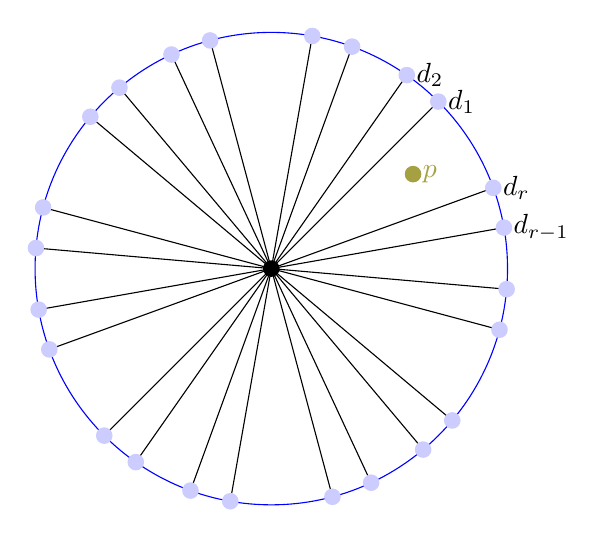
\begin{tikzpicture}[scale=3]
      \node[] (zero) at (0,0) {};
      \draw[blue] (zero) circle (1cm);

      \foreach \w/\str in {10/$d_{r-1}$,
                           20/$d_r$,
                           45/$d_1$,
                           55/$d_2$}
      {\draw (0,0) -- +({cos( \w )},{sin( \w )}) node[right] {\str};
       \fill[blue!20!white] ({cos( \w )},{sin( \w )}) circle (1pt);
       \foreach \sep in {60,120,180,240,300}
       {\draw (0,0) -- +({cos( \w + \sep )},{sin( \w + \sep )});
        \fill[blue!20!white] ({cos( \w + \sep )},{sin( \w + \sep )}) circle (1pt);
       }
      };

      \fill[yellow!60!black] (0.6,0.4) circle (1pt);
      \node[yellow!60!black,right] at (0.6,0.4) {$p$};

      \fill (zero) circle (1pt);
    \end{tikzpicture}
  \end{center}
  Label the first anti-Stokes ray when turning in a positive sense from $p$ as
  $d_1$ and label the subsequent rays $d_2,\dots,d_r$ in turn.
\end{frame}

\begin{frame}{Labeling convention (2)}
  \begin{center}
    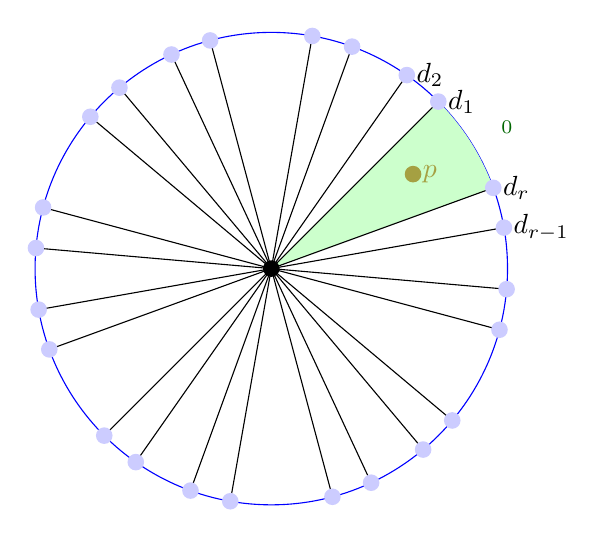
\begin{tikzpicture}[scale=3]
      \node[] (zero) at (0,0) {};
      \draw[blue] (zero) circle (1cm);

      \fill[fill=green!20!white] (0,0) -- ({cos( 20 )},{sin( 20 )}) arc
      (20:45:1) -- cycle;
      \node[green!40!black] at (1.0,0.6) {$\Sect_0$};

      \foreach \w/\str in {10/$d_{r-1}$,
                           20/$d_r$,
                           45/$d_1$,
                           55/$d_2$}
      {\draw (0,0) -- +({cos( \w )},{sin( \w )}) node[right] {\str};
       \fill[blue!20!white] ({cos( \w )},{sin( \w )}) circle (1pt);
       \foreach \sep in {60,120,180,240,300}
       {\draw (0,0) -- +({cos( \w + \sep )},{sin( \w + \sep )});
        \fill[blue!20!white] ({cos( \w + \sep )},{sin( \w + \sep )}) circle (1pt);
       }
      };

      \fill[yellow!60!black] (0.6,0.4) circle (1pt);
      \node[yellow!60!black,right] at (0.6,0.4) {$p$};

      \fill (zero) circle (1pt);
    \end{tikzpicture}
  \end{center}
  \begin{itemize}
    \item Write $\Sect_i:= \Sect(d_i,d_{i+1})$ the ‘ith sector’.
    \begin{itemize}
      \item Note $p \in\Sect_r= \Sect_0$
    \end{itemize}
  \end{itemize}
\end{frame}

\begin{frame}{Labeling convention (3)}
  \begin{itemize}
    \item $\widehat{\Sect}_i:=
      \Sect(d_i-\frac{\pi}{2k-2},d_{1+1}+\frac{\pi}{2k-2})$ the ‘ith supersector’
      \begin{itemize}
        \item The rays bounding these supersectors are usually refered as 
          \textcolor{red!40!black}{‘Stokes rays’}.
      \end{itemize}
  \end{itemize}
  \begin{center}
    \begin{tikzpicture}[scale=3]
      \node[] (zero) at (0,0) {};
      \draw[blue] (zero) circle (1cm);

      \fill[fill=green!20!white] (0,0) -- ({cos( 15 )},{sin( 15 )}) arc
        (15:85:1) -- cycle;
      \node[green!40!black] at (.9,.9) {$\widehat\Sect_1$};

      \draw[thick,red!40!black] (0,0) -- +({cos( 85 )},{sin( 85 )});
      \draw[thick,red!40!black] (0,0) -- +({cos( 15 )},{sin( 15 )});

      \foreach \w/\str in {10/$d_{r-1}$,
                           20/$d_r$,
                           45/$d_1$,
                           55/$d_2$}
      {\draw (0,0) -- +({cos( \w )},{sin( \w )}) node[right] {\str};
       \fill[blue!20!white] ({cos( \w )},{sin( \w )}) circle (1pt);
       \foreach \sep in {60,120,180,240,300}
       {\draw (0,0) -- +({cos( \w + \sep )},{sin( \w + \sep )});
        \fill[blue!20!white] ({cos( \w + \sep )},{sin( \w + \sep )}) circle (1pt);
       }
      };

      \fill[yellow!60!black] (0.6,0.4) circle (1pt);
      \node[yellow!60!black,right] at (0.6,0.4) {$p$};

      \fill (zero) circle (1pt);
    \end{tikzpicture}
  \end{center}
\end{frame}

\begin{frame}{Theorem 3.1}
  Suppose $\hat{F}\in G\llbracket z\rrbracket$ is a formal transformation such
  that $A:=F[A0]$ has convergent entries. Set the radius of the sectors
  $\Sect_i$, $\widehat\Sect_i$ to be less than the radius of convergence of
  $A$.
  Then the following hold:
  \begin{enumerate}
    \item On each sector $\Sect_i$ there is a canonical way to choose an
      invertible $n\in n$ matrix of holomorphic functions $\Sigma_i(\hat F)$
      such that $\Sigma_i(\hat F)[A^0]=A$
    \item $\Sigma_i(\hat F)$ can be analytically continued to the supersector
      $\widehat\Sect_i$ and then $\Sigma_i(\hat F)$ is asymptotic to $\hat F$
      at $0$ within $\widehat\Sect_i$
    \item If $g\in G\{z\}$ and $t\in T$ then 
      $\Sigma_i(g\circ\hat F \circ t^{-1})=g\circ\Sigma_i(\hat F)\circ t^{-1}$.
  \end{enumerate}
  The point is that on a narrow sector there are generally many holomorphic
  iso-morphisms between $A_0$ and $A$ which are asymptotic to $\hat F$ and one
  is being chosen in a canonical way; $\Sigma_i(\hat F)$ is in fact uniquely
  characterised by property 2.
\end{frame}

\begin{frame}{Functions on the quotient $\mathcal{H}(A^0)$}

\end{frame}

\begin{frame}
\end{frame}
